% What should the title be?
% Novelty Detection for Visual Indoor Categorization
% Novelty Detection on Semantic Representations.


\chapter{Introduction}
% Introduce:
%  Mobile Robotics, A.I.
%  Interaction with Humans
%  Need for concepts/semantic information
%  Dynamic human environment
%  Non-feasibility of hard-coded concepts
%  Requirements to detect novelty and handle it.
For a long time humanity has fantasized that one day robots will walk among us.
They will move and be able to interact with us. Understand our concepts and
be able to reason.

They need to possess ability to adapt to situations as its infeasible to rely
on extensive man-work to tag objects, map space and code all the aspects that
make up our human-reality.

% == Introduce the need of semantic representations ==
%
% There is a lot of low-level methods (or specific knowledge to robots)
% But the creation of semantic representations allow to bridge that low-level
% sensing with high-level concepts that facilitate several high-level Tasks.


% Importance of mapping and localization in a robot as well as reasoning on
% properties of each space.
% Humans give labels to space that characterized the properties and activities
% expected to be performed on them.
% Such information is of great interest to be structured and organized in such
% a way reasoning and planning can be implemented.
%
% It also holds an important role in long-term planning and stability as it
% hides the space-time local details and allows to focus on high-level thinking.

% Deal with uncertainty -> need for probabilistic models.
% Deal with semantic    -> need of structured models such as graphical models.


Example of what kind of an high-level thinking on space and its semantics can
provide: Get me a beer/milk concept.

% == Reasoning about need for Novelty Detection ==
%
% Dynamic environment (inability to know the environment or even to be possible
% to map all semantic concepts to interact with humans).
%
% Knowledge-Awareness (knowing what we know... And detecting novel cases)
% Identify gaps in the semantic knowledge.
% Automatic detection and learning of novel concepts.
%
% Increase robustness
% Self-Extending
%


\section{Problem and Goals}
% Extend a probabilistic graphical modelling framework with capabilities to
% detect novelty.
% Both in terms of novel classes as of novel structure.
%
Given a probabilistic structure representing the sensed conceptual knowledge
obtained by the agent develop methods able to detect novelty present
either on new semantic concepts (new classes) or even on structure that was
previously unknown.


% Yeah thats what you call dream :P
In an extreme ideal case the agent should be able to go from zero-knowledge to
understanding presence of certain objects (as generators of a set of sensed
sensed properties grouped locally), understand areas within rooms (sink-area on
on a kitchen), rooms as separated by doors, and understand environments such
as office, home, warehouse, spaceship.


For that the probabilistic semantic representation presented by
\cite{andrzej2011phd} is used.

% If everything goes fine... 2 of the "Future Directions" proposed are 
% Novelty Detection and Learning of Novel Concepts:
%  Identify Gaps in Spatial and Semantic Knowledge -> Addressed
%  Performing learning of new concepts -> Outside Scope / No Time
%
% Using Properties for Space Segmentation
%  If we move on detecting novel structures on the graph we are addressing this
%  issue.



\section{Thesis Outline}
The rest of this thesis is structured as follows:

\autoref{chap:background} introduces background concepts for understanding the
presented thesis. In particular \autoref{sec:graphical-models} introduces
\emph{probabilistic graphical models} that lay the base modelling tool for
the used structured semantic representation.

\autoref{chap:semantic-mapping} describes the system proposed by
\cite{andrzej}. In special it introduces the \emph{conceptual map} of the system
that is responsible for the creation of the \emph{probabilistic semantic
representation} that this thesis aims at improving by developing methods with
the capability to identify knowledge gaps.

\autoref{chap:novelty-intro} introduces novelty detection under a
statistical view point and how to interpret it as a threshold function.
A simple approach on how to perform novelty on very simple graphs
is given together with some results on the impact of using semi-supervised
novelty detection to improve the system performance.

\autoref{chap:novelty} presents the developed techniques developed to identify
novelty on the semantic representation.

\autoref{chap:conclusions} draws conclusions on the developed work and presents
interesting directions for future works.



%%%%%%%%%%%%%%%%%%%%%%%%%%%%%%%%%%%%%%%%%%%%%%%%%%%%%%%%%%%%%%%%%%%%%%%%%%
%%%%%%%%%%%%%%%%%%%%%%%%%%%%%%%%%%%%%%%%%%%%%%%%%%%%%%%%%%%%%%%%%%%%%%%%%%
\chapter{Background}
\label{chap:background}

In this chapter the background needed to understand the problem of visual place classification and novelty detection will be presented.
It should be enough to introduce several concepts to a reader unfamiliar with computer vision and machine learning areas.
And for readers seeking deeper detail all the concepts have been referenced to papers presenting them.

\section{Visual Place Classification}
\label{sec:place-classification}

\begin{figure}[here]
\begin{center}
\includegraphics[width=0.9\textwidth]{place_classification}
%\caption{Place classification deals with the problem of mapping a given location to a set of known concepts}
\end{center}
\end{figure}

Place Classification deals with the problem of mapping a given location to a set of known concepts.
In this thesis work its assumed the existence of labelled data (sample inputs where the correct label is known) that the algorithm can use during a training step, this is known as supervised-learning.
After the learning step the algorithm is feed with new data and is expected to guess the correct label.

It may feel natural then to pose the classification problem as a probability estimation problem of all the classes and pick the most likely. And several algorithms exists to perform that kind of analysis on data.
Though the problem of probability density estimation is harder than the problem of classification as it requires a full estimation over input space instead of a single decision between classes.
And one should not try to solve an harder problem.

So the usage of discriminative solutions, such as Support Vector Machines, is expected to lead to easier solutions.

There exists several methods that can be used for classification problem such as usage of \emph{Neural Networks}, \emph{Nearest-neighbours}, \emph{Decision Trees}, \emph{Bayesian Networks} and other statistical tools for regression and statistical analysis.
Though since only \glspl{SVM} are used on this work only a short overview over them is provided. For extended knowledge in the methods the reader is advised to look on other materials~\citep{bishop2006pattern}.

\subsection{Support Vector Machines}
\Glspl{SVM} where introduced by \cite{cortes1995support} and can be seen as discriminative linear based classifier.
They are based on a strong mathematical foundation and have powerful generalization capabilities.
In their original form \gls{SVM} separates two classes of points in an hyper-space with a \emph{maximal margin hyperplane}~(\autoref{fig:svm-sample}).

Later they were extended to deal with noisy data by using \emph{soft margins}.
And to handle non-linear spaces as seen on \autoref{sec:kernel-trick}.
Although they only allow for two class-classification several methods have been proposed to build multi-class classifiers based on binary classifiers as seen on \autoref{sec:multiclass-classifiers}.

\begin{figure}[h]
\begin{center}
\includegraphics[width=0.5\textwidth]{Svm_max_sep_hyperplane_with_margin}
\end{center}
\caption{{SVM} separating two class of points by a \emph{maximal margin hyperplane}. The hyperplane can be described by the collection of support vectors and associated weights, marked in the image as sample points with large borders.}
\label{fig:svm-sample}
\end{figure}

They have been used in several classification and recognition problems and are in fact a standard across machine learning techniques.
Their efficiency, exact training results and generalization made their suitable for many tasks. Such as text categorization, digit-recognition, spam-classification.
They have also been extensively used in visual place classification~\citep{pronobis2005msc}.

\subsection{The Kernel Trick}
\label{sec:kernel-trick}
\gls{SVM} in their basic form are only able to handle linear spaces.
Nonetheless the classes are most of the time not linearly separable in the input space.
Although there might exists a transformation $\phi$ from the original space into a space $H$ where the input becomes linearly separable.

The Kernel trick allows to extend the \gls{SVM} definition to work on such space $H$ without ever performing an implicit transformation between spaces.
Being enough for that to have a Kernel function defining an inner-product inside such space: $K(x_i, x_j) = \phi(x_i)\cdot\phi(x_j)$.
In that sense a Kernel function can be seen as a function that calculates some similarity measure between two inputs.

Several kernel functions have been proposed being the most commonly used:

\begin{description}
\item[Polynomial Kernel] - $K(x, y) = (x \cdot y + p)^d$
\item[Radial Basis Function] - $K(x, y) = e^{-\gamma\|x - y \|^2}$
\item[Histogram intersection] - $K(x, y) = e^{-\gamma \chi^2(x,y)}$, where $\chi^2(x,y) = \sum_{i=1}^{N}\frac{(x_i-y_i)}{x_i+y_i}$ introduced by \cite{barla2003histogram} allows to compute histogram similarity.
\item[Matching Kernels] - mimic matching similarity and are used when each sample is represented as a set of features~\citep{boughorbel2005intermediate}.
\end{description}

\subsection{Extending to Multi-class}
\label{sec:multiclass-classifiers}
\Glspl{SVM} were designed as two-class classifier. And so they need to be adapted for using in multi-class problems.
The most common usage is to design multi-class classifiers recurring at the usage of multiple two-class classifiers and methods for combining them.
The most typical approaches for a multi-class classification on $c$ classes using \glspl{SVM} are:

\begin{description}
\item[One Against All] - in this method $c$ distinct classifiers are trained to distinguish any class of the remaining ones.
The output of all those classifiers (distance to the separating hyperplane) is then used to categorize the output.
The most common approach is to pick the class with the largest hyperplane distance.
Other variations exists as is the case of using the minimal distance to the average classification distance of each class~\citep{pronobis2007confidence}.

\item[One Against One] - in this method $c*(c-1)/2$ classifiers are trained to distinguish between each pair of classes. The final decision is based on the output of all those classifiers being common to use a majority vote strategy.
\end{description}


\subsection{Features}\label{sec:features}
A feature is a piece of information which is expected to reveal information for solving a specific task.
In that sense features are task-dependant and they will yield different performance based on the type of task they are applied to.

A wanted property on features is its repeatability under similar conditions for the problem in hand. This is: they should be stable and invariant across unwanted types of transformations and noise.
For example a visual feature for object detection should be present even if the target object was translated, scaled, rotated, the light-conditions have changed or even if the object is partially occluded.

Extracting features with those properties allows to greatly reduce the size of input by removing unwanted noise and useless information from the captured data.
Turning the classification problem easier, more reliable and more efficient.

Often several and different types of features need to be extracted. It has been reported by \cite{pronobis2010ijrr} that using multiple features provides a great benefit in the context of place classification.
And \cite{quattoni2009recognizing} has showed that different types have different impact in indoor scene recognition based on the type of scene matching.
Namely was seen that some room-categories are more likely to be recognized by the presence of some objects and others by it generic appearance.

In the context of robotics, sensors such as cameras, laser scans are used to sense the surrounding environment, and features can be extracted from all those. Nonetheless as described in \autoref{sec:visual_motivation} the visual sensor is incredibly rich and most of our features will come from it.

Visual features can be seen as belonging to two categories: \emph{local features} and \emph{global features}.
\emph{Local features} describe fine grain properties of a part of image. For example the existence of specific corner or an edge. \Gls{SIFT} (\autoref{sec:sift}) is an example of such feature and has been proven useful for matching points between images and subsequence extension to object detection.

\emph{Global features} such as \gls{CRFH} (\autoref{sec:crfh}) or {gist}~(\autoref{sec:gist}) try to describe the whole image. Either by statistical analysis of features over all the image or by a structured distribution of textures findable in the image.

\subsubsection{{SIFT} - Scalar Invariant Feature Transform}
\label{sec:sift}\label{sec:local-features}
The detection of interesting points has been studied for several years and is the base of several computer vision problems solution. It allows to perform point matching which can be used in several areas from image stitching, 3D reconstruction, video tracking, object detection, etc\dots

The most used method was presented by \cite{lowe1999object}. And its based on building a feature vector for each image. Each of those features is based on \emph{interesting points} detected by detecting maxima and minima of a difference of Gaussian functions applied in a scale-space.
The scale space is used to provide scale invariant detection. Gaussian functions are used as they are the only way to model a linear scale-space.
Each interesting point is then described by a contained that is rotation invariant.

By seeing an object as a set of features points, index and matching is then performed by a high-dimensional search on a database of know objects. After matching objects can be verified for geometric coherence between features.
\Gls{SVM} classifiers can also be trained to detect objects based on this type of local features by using \emph{Matching kernels} (\autoref{sec:kernel-trick}).

\begin{figure}[h]
    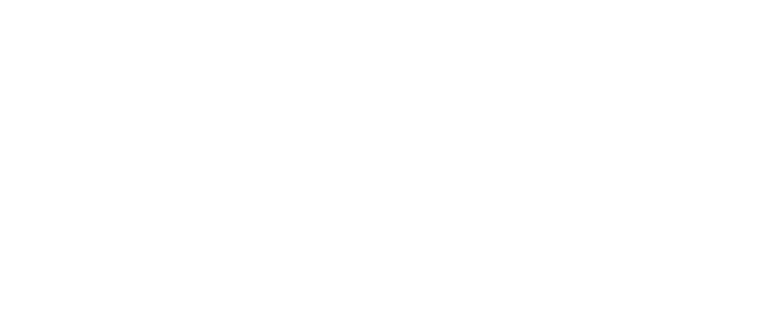
\includegraphics[width=\textwidth]{sift/sift.pdf}
    \caption{{SIFT} and other local features have been proven useful in object detection.}
\end{figure}


\subsubsection{Gist of a Scene}
\label{sec:gist}
\cite{oliva2006building} argue that fast scene recognition does not need to be built on top of object recognition but can be analyzed by scene-centered mechanisms.
They defend that position by pointing out behaviours on human vision:
when provided with a glance of a shot a person can identify the meaning of that given shot or "gist of a scene" without remembering specific details.

\begin{figure}[h]
\center
\includegraphics[width=0.60\textwidth]{gist.jpg}
\caption{An illustration of the gist of an image. Top row: original image I; bottom row:
noise image J for which gist(I) = gist(J). We see that the gist captures the dominant
textural features of the overall image, and their coarse spatial layout~\citep{murphy2006object}.}
\end{figure}


\subsubsection{{CRFH} - Composed Receptive Field Histograms}
\label{sec:crfh}\label{sec:global-features}
Composed Receptive Field Histograms are a multidimensional statistical representation of the occurrence of several image descriptors applied to an image.
They can be seen as an high-dimension histogram where each cell records how many pixels of the image have the cell response for the applied descriptors.
Such high-dimensional histogram is expected to be able to better global information contained in the image by capturing several properties of the image as well the relations between them.


\begin{figure}[h]
\begin{center}
\includegraphics[width=1\textwidth]{crfh_model.jpg}
\end{center}
\caption{A two dimensional histogram of the image built out from two image descriptors: $Lx$ and $Ly$. First-order Gaussian derivatives of image luminance in horizontal and vertical direction applied at a scale 4.}
\end{figure}

Several type of image descriptors can be applied.
For example Gaussian derivatives (such as $L_x$, $L_y$, $L_{xx}$, $L_{yy}$) are partial derivatives of the image luminance after applying a Gaussian filter of a given scale ($\sigma$) on the image.
Gradient magnitude descriptors (such as $|\nabla L|$) can also be used as a rotation invariant descriptor.


One of the problems of high-dimensional histograms is the memory and computationally complexity needed to handle them.
\cite{linde2004object} suggested using a sparse form to represent those by storing only the non-zero-cells in an array structure.

Multidimensional histograms have proven to be useful in the context of object recognition~\citep{schiele1996object}. And have also been previously used in the context of visual place classification~\cite{pronobis2010ijrr}.
\emph{Histogram intersection kernels} (\autoref{sec:kernel-trick}) can be used to train classifiers based on this feature.


\subsection{Other features}
Robots are often equipped with other types of sensors besides cameras and those can be used to extract information from the surrounding environment and yield useful information for the problem of place classification.

An example of such a sensor is a laser scan. Many robots are equipped with them and use it for low-level navigation.
From them its possible to extract a few set of geometric features, such as elongatedness ratios, or room size, which definitely yield important information for place classification.

Currently, with the deploy of the \gls{Kinect} device there has been an increasing usage of depth information available.
We expect that very soon usable features from that type of sensors will be developed.

\begin{figure}[h!]
\center
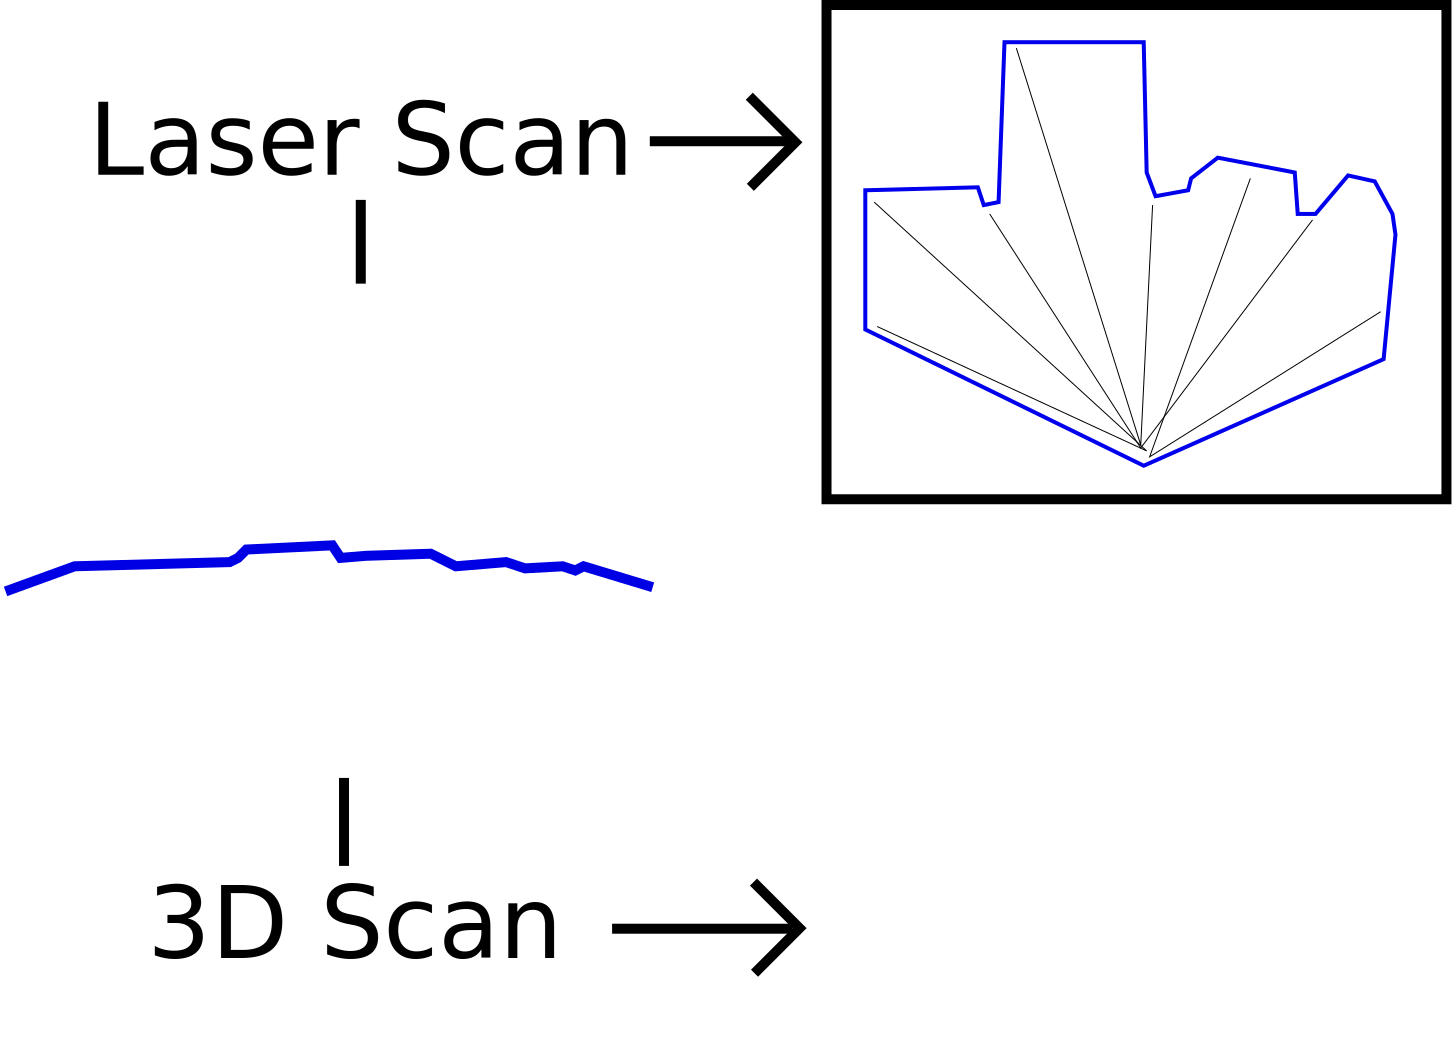
\includegraphics[width=0.5\textwidth]{laser_and_depth_input.pdf}
\caption{Using current laser sensors its possible to extract both 2D and 3D depth information from the environment.}
\end{figure}

\subsection{Spatio-temporal Accumulation}
\label{sec:accumulation}
In the context of robotics, data is not only available as a single-instant (eg.: single frame) but its acquired across time and space as the robot moves through the environment.
This can be used to further improve place classification by accumulating the several clues extracted by the robot for a given position and time.

By using odometry data (such as position and heading) its possible to create a view-point dependent histogram of the robot observations, which can be integrated using discriminative techniques and confidence level estimations. This approach greatly increases the reliability of classification methods as turns the classification more robust against noise or unbalanced data (such as a robot staring at a wall). \cite{pronobis2010ijrr} uses this technique.


\newpage
\section{Novelty Detection}
\label{sec:novelty-detection}
Novelty detection, also called outlier or anomaly detection, is the classification problem related with identification of new or unknown data that the system was not aware of during the training.

It has several applications such as fault detection, intrusion detection, detection of masses in mammograms, hand written digit recognition and many others~\citep{markou2003novelty}.
And has seen an increase of its application in the area of robotics and control.

It is posed as a one class classification where there is only access to the positive samples.
The objective then is to classify new inputs as being generated by the class it was trained or if they belong to some new unknown one.

Either by impossibility of generating samples of "unknown", or by extreme difficulty to acquire negative-examples, two-class classifiers cannot be applied to this problem.
Several other methods were developed to address this problem and they often can be categorized in the following approaches:
based on probability density estimation;
based on using the feature space to separate the given class from others, such as one-class \gls{SVM};
and based on reconstruction-error from a lower-dimension.


\subsection{Density estimation}
One of the simplest approach for novelty detection is pose the problem as a probability density estimation problem and use the expected probability of a given input to trigger the case as novel.

Examples of such approaches are Gaussian Mixtures Models and Parzen-window estimators.
In order to reduce the input size, those approaches often employ dimension-reduction techniques such as \gls{PCA}.

This approach is used in \cite{bishop1994novelty} where \emph{novelty detection} is added to a \emph{neural network} system.
On it the density estimation on the input is calculated using a \emph{Parzen window} over training-data and that value is used as a novelty measure. This way they detect novel data that the their network has not seen before and so the expected output of their system is not reliable.

\subsection{One-class {SVM}}
One-class \gls{SVM} approaches try to distinguish the class by separating the training set from all other points in the input space. They try to archive that by enclosing the training set by some structure (example: hyper-sphere)~\citep{scholkopf2000support}.
This leads to a decision boundary and follows the same principal as Vapnik solving classification with \gls{SVM}: do not solve something harder.

\subsection{Reconstruction Error}
Error reconstruction methods for novelty detection use the assumption that the class to be defined lies on a manifold embedded on the input space of higher dimensions.
By using dimensional reduction techniques, they try to defined that manifold and calculate how far a new input is from it.

\label{sec:kernel-pca}
One of the most common methods used for that is \gls{K-PCA}~\citep{scholkopf1997kernel}, which uses the kernel-trick (\autoref{sec:kernel-trick}) to extend \gls{PCA} and perform a nonlinear dimensionality reduction on the input. This technique has been successfully used in novelty detection by \cite{Hoffmann2007863}.

\begin{figure}
\center
\includegraphics[width=0.50\textwidth]{ringlinesquare_kpca}
\caption{{Kernel PCA} used on a ring-square-circle distribution~\citep{Hoffmann2007863}.}
\end{figure}

\section{Graphical Models}
\label{sec:graphical-models}
Graphical models usage can be tracked back to earlies 1920 but they only become popular in mid-eighties when researchers started to use \emph{Bayesian Networks} to model expert systems~\citep{borgelt2002graphical}.

They serve as a better tool to model \emph{random variables} (nodes on the graph) and their probabilities as they model the conditional dependence between variables (edges on the graph).
Important to note that here \emph{random variables} does not denotes a truly random variable but one that is unknown by the system and is conditioned by other variables/evidences.

This type of graphs provide a generative model where the probability of any given scenario can be determined. As opposed to non-generative models where a given probability can only be calculated if certain data is given.
This means when a graphical model is learned, it can be used to generate new samples from the learned distribution.

They have been successfully used in several machine-learning task such as: information extraction, speech recognition, computer vision. They are also useful due to their ability to deal with semantic (high-level) features~\citep{boutell2006factor} and ability to represent properties of the reality they try to model.

Two main types of graphical models have been used: Bayesian Networks which model directed edges between variables and Markov Random Fields where variables are connected by a potential but no special direction is given to edges.

An important property of these graphs is the \emph{Markov-blanket} of a node.
For a given variable $a$, a \emph{Markov-blanket} is a set of variables in the surroundings of $a$ that when given the value of $a$ becomes independent of the rest of the graph~\citep{pearl1988probabilistic}.
On non-directional graphs it is directly determined by the nodes connected to $a$.
This allows the usage of graph algorithms such as \emph{min-cut} to quickly determine most likely scenarios.
In the case of directed edges a node blanket is also influenced by the direction of the edges and a more complex schemes need to be used.

As \cite{lauritzen2002chain} points this two types of models can be represented as a \emph{chain graph} where both directed and undirected edges can co-exist.
Though this generalization is hard to implement due to mis-understandings on the concepts the graph-models use.

Another useful interpretation of graphical-models are \emph{factor graphs}. Those are able to handle both \emph{Bayesian Networks} and \emph{Markov Random Fields}. Under this interpretation a graph is seen as a bipartite graph that connects variables with factors that influence them~\citep{bishop2006pattern}.
This gives a very useful framework to develop belief propagation on them by seeing a message-passing mechanism between nodes. Belief propagation is used to calculate marginal-probabilities.

\begin{figure}[ht]
    \begin{minipage}[b]{0.3\linewidth}
        \centering
        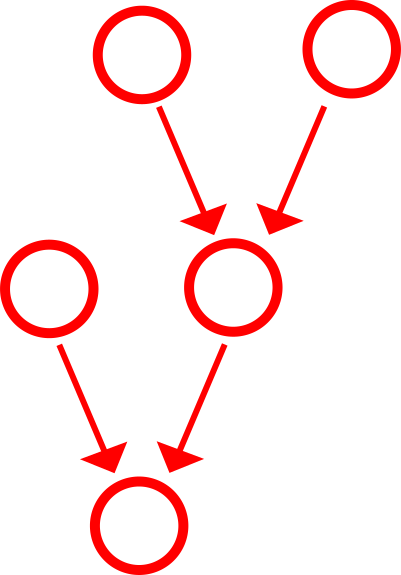
\includegraphics[width=0.8\textwidth]{graphical-models/BayesNet.pdf}
        \caption{Bayes Networks}
    \end{minipage}
    \hspace{0.5cm}
    \begin{minipage}[b]{0.3\linewidth}
        \centering
        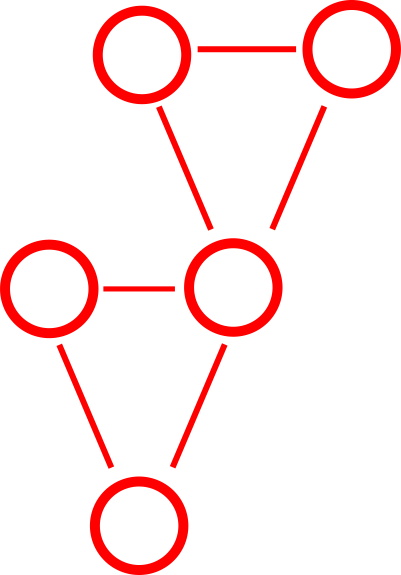
\includegraphics[width=0.8\textwidth]{graphical-models/MarkovRandomField.pdf}
        \caption{Markov Random Field}
    \end{minipage}
    \hspace{0.5cm}
    \begin{minipage}[b]{0.3\linewidth}
        \centering
        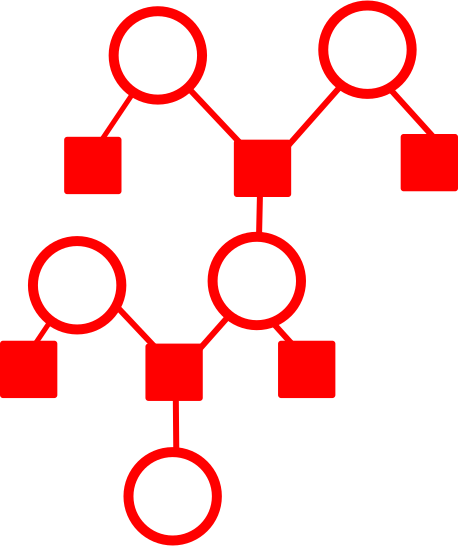
\includegraphics[width=\textwidth]{graphical-models/FactorGraph.pdf}
        \caption{Factor Graph}
    \end{minipage}
\end{figure}


%%%%%%%%%%%%%%%%%%%%%%%%%%%%%%%%%%%%%%%%%%%%%%%%%%%%%%%%%%%%%%%%%%%%%%%%%%
%%%%%%%%%%%%%%%%%%%%%%%%%%%%%%%%%%%%%%%%%%%%%%%%%%%%%%%%%%%%%%%%%%%%%%%%%%
\chapter{Semantic Mapping}\label{chap:semantic-mapping}

% Advantages of Multi-modal approaches
% 

\section{Dora Architecture Overview}
\subsection{System organization}
\subsubsection{Sensory Layer}
\subsubsection{Categorical Layer}
\subsubsection{Place Layer}
\subsubsection{Conceptual Layer}

\section{Features}
\section{Conceptual Knowledge}
\section{Conceptual Map}

%%%%%%%%%%%%%%%%%%%%%%%%%%%%%%%%%%%%%%%%%%%%%%%%%%%%%%%%%%%%%%%%%%%%%%%%%%
%%%%%%%%%%%%%%%%%%%%%%%%%%%%%%%%%%%%%%%%%%%%%%%%%%%%%%%%%%%%%%%%%%%%%%%%%%
\chapter{Novelty Detection}\label{chap:novelty-intro}

This chapter presents the main work of this thesis: a method to augment the conceptual
map with novelty detection capabilities.

The chapter starts by providing the reader with a brief overview on novelty detection
techniques and related works. Then it shows that an optimal novelty detection system
can be implemented by thresholding on a order-relation defined over the inputs.
And that an equivalent order-relation can be imposed by a ratio between
conditional and unconditional probabilities.
Some discussion on how to interpret the meaning of those factors is also
presented.

At last a practical example using semantic data and probabilistic graphical
models is presented: it shows how to use the introduced ratio to obtain a
novelty detection system and analyses the performance impact by increasing
the amount of sensed data and by using an approximation on the unconditional
probability.


\section{Novelty Detection Review and Related Work}
Novelty detection, also known as outlier or anomaly detection, is a
classification problem related to identification of new or unknown data
patterns that the system is not aware of~\cite{markou2003novelty}.

The ability to identify novel cases is crucial in any autonomous system
that is deployed to unknown or to uncontrolled environments, as it gives the
system the ability to detect that something is not conforming to its knowledge and
therefore should be treated with caution.
It has several applications such as fault detection~\cite{tarassenko1999novelty},
intrusion detection~\cite{fan2001using},
detection of masses in mammograms~\cite{tarassenko1995novelty} or detection of
novel and useful documents~\cite{zhang2002novelty}.

Any normal classification application is also a good candidate for extending
with novelty detection, as the results for samples the system has not been
trained on can be unreliable~\cite{devarakota2008reliability}.
e.g.\ applied to digit-recognition~\cite{tax1998outlier}
or to detection of novel inputs on a neural network~\cite{bishop1994novelty}.

It is in the nature of unknown environments and in the infeasibility of
the system to acquire examples of all possible classes where the complexity of
novelty detection lies: it is only possible to obtain samples representing positives
examples of known cases and the lack of negative examples renders normal
classification methods unusable.
In order to become practical in real world applications, novelty detection
methods have to overcome a series of obstacles:
be able to generalize while still detecting novelty,
be resistant to noisy features,
ability to scale in feature dimension,
deal with multiple classes and performing detection efficiently as many
autonomous systems require real-time or close to real-time performance.

\subsection{Review of Novelty Detection Methods}
A common approach is to use density estimation and use the expected probability
of a sample to classify the sample as novel. Examples of such techniques are
Gaussian Mixture Models and Parzen-window estimators. In order to be effective,
those rely on data as close as possible to the input features and use
dimensionality\hyp{}reduction techniques such as \gls{PCA} to make density
estimation feasible. Note that as dimension increases an exponential number
of data samples would be required to approach the density with the same quality.

\cite{bishop1994novelty} uses that approach by employing a Parzen-window to
estimate the density of the training data on a given input fed into a
neural-network. Using the calculated density, they detect samples
that differ from the training data and consider their neural-network output
to be unreliable as the samples are distinct from what the network was trained
with.

A slightly different approach is applied in case of by one-class \gls{SVM} approaches that
try to distinguish novelty by separating the training set from all the other
points in the input space. They try to achieve that by enclosing the training
set by some structure (e.g.\ an hyper-sphere)~\cite{bennett2000support}.
Those approaches have been made in line with Vapnik principle of not solving
something hard. As although having access to a perfect probability distribution
of the input would solve the problem, creating such a function is harder than
simply creating a boundary between known data and novel data
\cite{scholkopf2000support}.

Error reconstruction methods have also been used for novelty detection.
They use the assumption that the class to be defined lies on a manifold embedded
into a sample space of higher dimensionality. By using dimensionality\hyp{}reduction
techniques, a manifold is defined and the distance between the manifold and the new sample
is calculated. One of the most common methods used for that purpose is
\gls{K-PCA}~\cite{scholkopf1997kernel}, which uses the kernel-trick to extend
\gls{PCA} and perform a nonlinear dimensionality reduction of the input.
This technique has been successfully used for novelty detection in \cite{Hoffmann2007863}.

\cite{japkowicz1995novelty} also follows a similar approach: \emph{Redundancy
Compression and Non-Redundancy Differentiation} which is a process believed
to happen in the hippocampus. They introduce an auto-encoder
that learns to encode a sample on a considerable smaller description and later reconstructs
the original sample from this smaller description. Their suggested system
learns how to discard and compress redundant information while still be able to recover
the original sample. By training it with samples from a given class, it
is expected that it will badly reconstruct a sample from a different one.

\cite{ranganathan2010pliss} presents a system able to perform place recognition
and classification from visual clues. It is able to perform segmentation by
exploiting time-coherency on video information. The approach is particularly
interesting by its ability of keeping a fully probabilistic distribution of
the place classification and segmentation. This is, the system never performs
a deterministic decision that impacts any future result, allowing it to adjust
the segmentation and place classification as more data becomes available.
The system is also able to detect novel instances and methods how to adapt it
to run on a constant amount of memory and computation are presented.

\cite{boutell2006factor} presents a method to perform scene-classification
from low-level region detectors using probabilistic graphical models.
The information obtained by the region detectors is exploited together with the
spatial relations between on the higher level scene-classification task.
A presented scheme using only pairwise relations between regions is show to
have better performance than the correct approach of modelling all regions connectivity
with a large single-factor as the pairwise relations can be
approximated with modest amounts of training data, where the single-factor
demands an impractical amount of training data.
No approach is made on it at novelty detection either of regions or scene
categories. 


\section{Novelty Detection by Thresholding}
\label{sec:threshold}
The objective of a novelty detection system is to classify a given sample $x$ as
either \emph{known}: $x$ being generated by a known class to the system, or \emph{novel}:
$x$ generated by a class unknown for the system.
Based on the ground\hyp{}truth of a sample four cases are possible:

\begin{description}
\item[true positive]  - when a system correctly   flags a sample of an unknown class as \emph{novel}.
\item[false positive] - when a system incorrectly flags a sample of a known class as \emph{novel}.
\item[true negative]  - when a system correctly   flags a sample of a known class as \emph{known}.
\item[false negative] - when a system incorrectly flags a sample of an unknown class as \emph{known}.
\end{description}

Due to noisy data, unstable features and lack of information it is impossible to develop
a method able to exactly guess the correct classification of a sample.
By modelling the outcomes with probabilities it becomes possible to handle the uncertainty
associated with each decision.
The notation $P(novel|x)$ will be used to denote the probability that the sample $x$ is in fact a
sample of an unknown class. $P(x)$ will denote the probability that sample $x$ is given to the
system to be classified. $\overline{novel}$ is also defined in such a way that
$P(\overline{novel}|x)$ measures the probability that a decision on classifying $x$ as novel is
wrong.

Additionally a decision on the novelty of a sample $x$ performed by a deterministic system
will be fully determined by the sample itself.
Which implies that any deterministic novelty detection system can be uniquely determined by the set $N$
of samples that are accepted by the classifier as \emph{novel}.
This way it is possible to define the probability of a true positive and false positive event for any
deterministic novelty detector with the following equations:

\begin{eqnarray}
P(\text{true positive})  &=& \sum_{x \in N}{P(novel|x)P(x)} \\
P(\text{false positive}) &=& \sum_{x \in N}{P(\overline{novel}|x)P(x})
\end{eqnarray}

Note that since probability functions are non-negative, it is impossible to decrease either the
true positive or the false positive probability by using a set $N' \supset N$.
This describes the base of the \emph{error and rejection tradeoff}~\cite{chow1970optimum}, which
states that a system aiming at increasing the true-positive probability will eventually increase its
false-positive error.
The true positive probability can be described as the interest in detecting as much
as possible the novel classes and the false positive probability the interest
in not incurring in too many errors.
By fixating one of those it is possible to define a novelty detection
system that achieves the maximum or minimum of the other.

This way an optimal detector can be formulated by achieving the maximum true-positive
probability without its false-positive probability increase beyond a given limit.
This is equivalent to a \emph{continuous knapsack problem} which allows a greedy
solution by sorting the items with a value per weight function.
In the case of detection system that can be defined as:

\begin{eqnarray}
value(x)  &=& P(\text{true positive}|x) \\
weight(x) &=& P(\text{false positive}|x) \\
cost(x)   &=& value(x)/cost(x) \\
          &=& \frac{P(novel|x)P(x)}{P(\overline{novel}|x)P(x)}
\end{eqnarray}

Therefore a novelty system before classifying a sample $a$ as novel should (greedily)
classify any sample $b$ with a small cost as that would achieve
an higher true positive probability given a fixed false positive one.

\begin{equation}
\label{eq:knapsack}
\frac{P(novel|b)}{P(\overline{novel}|b)} < \frac{P(novel|a)}{P(\overline{novel}|a)}
\end{equation}

This relation between $a$ and $b$ can further be simplified into:

\begin{equation}
P(\overline{novel}|b) < P(\overline{novel}|a)
\end{equation}


Based on this, it can be said that an optimal novelty detection system is
interested in defining an order relation on all the possible inputs equivalent
to the order defined by the function: $P(\overline{novel}|x)$.
And any optimal detector can be described by the largest $P(\overline{novel}|x)$
accepted by it. Which is seen as threshold.


\section{Conditional and Unconditional Probability Ratio}

On the previous section it was shown that an optimal novelty detector can be
implemented with a threshold on top of the order-relation defined by
$P(\overline{novel}|x)$ over $x$. Performing some manipulations with
Bayes theorem and assuming a constant $P(\overline{novel})$ a more usable
form can be attained:

\begin{equation}
\label{eq:novelty-ratio}
          P(\overline{novel}|x)
  =       \frac{P(x|\overline{novel}) P(\overline{novel})}{P(x)}
  \propto \frac{P(x|\overline{novel})}{P(x)}
\end{equation}

Since there is only interest in maintaining the same order-relation as
$P(\overline{novel}|x)$ any constant factor can be dropped.
Leaving a ratio between a \emph{conditional} and
\emph{unconditional probability} suitable for implementing novelty detection
by thresholding.


\subsection{Conditional Probability}
The conditional probability $P(x|\overline{novel})$ describes the distribution
of the samples given that they are generated by a known class.
In case the labelled data available for the agent to learn a concept comes from
the same distribution where the system will run the correct approach is to use it
as prior-information for modelling the conditional probability.

Note that it is important for the labelled data to be a filtered version
of the underlying world distribution (with all classes) that does not contains
any bias.
Otherwise that bias will lead to incorrect modelling the conditional probability
and a subsequent wrong ordering of the sample space.

\subsection{Unconditional Probability}
The unconditional probability $P(x)$ plays an important role on obtaining a
correct order relation for performing novelty detection.
It serves as a normalizing component that allows the system to figure out
whether a given sample conditional probability arises from it belonging to
the known concept or from the likelihood of being sampled.

On lack of any information about the unconditional probability and conforming to
the principle of maximum entropy (\autoref{sec:max-entropy}) a uniform
distribution must be chosen.
Though by using unlabelled data it becomes possible to obtain extra information
and achieve a better approximation.


%\subsection{Novelty Detection on a Variable Set of Features}
Note also that often novelty detection is applied on a fixed set of features
together with an assumption of a uniform unconditional probability.
On those cases $P(x)$ becomes a constant and therefore a novelty threshold
can be directly applied on $P(x|\overline{novel})$ as is the case in \cite{bishop1994novelty}.
But in the case where the set of features $x$ is variable it cannot be
discarded. There $P(x)$ plays a role in levering all the conditional
probabilities on different sets of variables into the same measure units
such that a threshold can be implemented.

\subsection{Assumption on a constant $P(novel)$}
The ratio between the conditional and unconditional probabilities of the sensed variables
is only directly applicable to novelty detection under the assumption of a constant $P(novel)$.

All the literature focus on novelty detection within a fixed scenario, where the set of variables
used to model the distribution is fixed and defined at the moment the threshold is trained.
Due to that, they can drop a constant $P(novel)$ and never need to directly or indirectly calculate
it.
To the best of the author knowledge there has not been studies on how to approximate it on dynamic
sets and structures of sensed variables, and so a strong assumption on being constant through all
the possible scenarios is used to allow dropping the factor.

This assumption was considered questionable on whether it holds on a realistic scenario,
and for that a sampling scheme able to comply with it is now presented as well an unbiased sampling
scheme. A method to generate samples that match this \emph{criterium} of having a constant $P(novel)$ can be:

\begin{algorithm}[Draw samples with equal $P(novel)$]
\begin{enumerate}
\item Sample a graph structure $G$ (where variable $a$ can be any of the known or unknown classes)
\item Decide novelty of $a$.
\item Sample the remaining variables according to distribution $P_G(x|a)$.
\end{enumerate}
\end{algorithm}

According to this sampling algorithm, given any structure the probability of
variable $a$ being novel is constant. This is somehow unexpected as it means
the sampling method is biased to adjust the real distribution $G$ such that
exactly a constant percentage of drawn samples are novel.

Alternative, the sampling method described below is considered more correct as
it introduces no bias on the distribution $G$ describing the real distribution
and classes of $a$:
\begin{algorithm}[Draw samples with equal $P(novel)$]
\begin{enumerate}
\item Sample a graph structure $G$ (where variable $a$ can be any of the known or unknown classes)
\item Sample variables $x$ according to distribution $P_G(x)$.
\end{enumerate}
\end{algorithm}

Due to the highly bias needed to drawn a constant amount of novel sampes from any structure, the
author defends this assumption to be very strong and points that future work should avoid.

 
%%%%%%%%%%%%%%%%%%%%%%%%%%%%%%%%%%%%%%%%%%%%%%%%%%%%%%%%%%%%%%%%%%%%%%%%%%%%%%%%%
%%%%%%%%%%%%%%%%%%%%%%%%%%%%%%%%%%%%%%%%%%%%%%%%%%%%%%%%%%%%%%%%%%%%%%%%%%%%%%%%%
\section{Novelty Detection on the Conceptual Map}

This section presents now how to use graphical models produced by the conceptual map and the
novelty detection concepts introduced earlier on this chapter in order to detect room categories the
system is not aware of.

For that both models to approximate both the conditional and unconditional probability need to
be defined and then the ratio between them used to define a function over which a threshold
implements a novelty detection system.

\subsection{Approximating the Conditional Probability}
The actual semantic mapping of the environment happens using the \emph{conceptual map}
introduced on \autoref{sec:conceptual-map}. During it the agent instantiates a
\emph{chain graph} to model distribution of the sensed variables according to the known
concepts and categories introduced as hidden variables on the graph. Using that graphical model
the system is able to propagate and find the most likely configuration of the represented
variables. For instance, the semantic category of a specific room is modelled as an hidden variable
with states representing the semantic values, by calculating probabilities on that variable the
system finds its belief on the room belonging to a specific category.

Since the graphical model produced by the conceptual map tries to model the distribution of
variables assuming the knowledge of the agent holds true, it represents a method to model
$P(x|known)$ since it allows to calculate the density probability that the set of features $x$ is
sensed given that all the variables and graph structure, including the category of
a specific room $a$ are correctly modelled by the agent knowledge.
This way the distribution modelled by a factor graph equivalent to the chain-graph used by
the conceptual map can be used as an approximation for the conditional probability of $x$.

\begin{figure}[h]
\centering
\begin{tikzpicture}
  \node [matrix,matrix anchor=mid, column sep=15pt, row sep=10pt,ampersand replacement=\&] {
    \& \& \node (room3) [latent] {}; \& \\
    \& \& \& \\
    \&
    \node (room1) [latent] {$a$}; \& \&
    \node (room2) [latent] {}; \\
    \& \& \& \\
    \node (shape1f) [factor] {}; \&
    \node (appearance1f) [factor] {}; \&
    \node (object1f) [factor] {}; \&
    \node (factor2) [factor] {}; \\
    \node (shape1l) [obs] {$S_p$}; \&
    \node (appearance1l) [obs] {$A_p$}; \&
    \node (object1l) [obs] {$O_p$}; \&
    \node (prop2) [obs] {$X_p$}; \\
  };

  \draw [-] (room1) -- (shape1f) -- (shape1l);
  \draw [-] (room1) -- (appearance1f) -- (appearance1l);
  \draw [-] (room1) -- (object1f) -- (object1l);
  \draw [-] (room2) -- (factor2) -- (prop2);

  \draw [-] (room1) -- (room2) node (r12f) [midway,factor] {};
  \draw [-] (room1) -- (room3) node (r13f) [midway,factor] {};
  \draw [-] (room2) -- (room3) node (r23f) [midway,factor] {};

  \begin{pgfonlayer}{background}
    \plate{places1}{(shape1f)(shape1l)(object1l)}{$\forall p \in places(room1)$}{};
    \plate{places2}{(factor2)(prop2)}{$\dots$}{};
  \end{pgfonlayer}
\end{tikzpicture}

\caption{Factor graph modelling the conditional probability distribution, case where the
         room category of room $a$ is known by the system.}
\end{figure}


\subsection{Approximating the Unconditional Probability}

With no knowledge on the unconditional probability the correct approach is to
assume a uniform distribution (\autoref{sec:max-entropy}), which can be modelled by a
factor graph without any factors: \autoref{fig:uniform-graph}.

\begin{figure}[h]
\centering
\begin{tikzpicture}
  \node [matrix,matrix anchor=mid, column sep=20pt, row sep=10pt,ampersand replacement=\&] {
    \node (x1) [obs] {$S_1$}; \&
    \node (x2) [obs] {$A_1$}; \&
    \node (x3) [obs] {$O_1$}; \&
    \node (xi) [] {\dots}; \&
    \node (xn) [obs] {$X_n$}; \\
  };
\end{tikzpicture}
\caption{\label{fig:uniform-graph}A factor graph modelling a uniform
         distribution over the sensed set of features $x$.}
\end{figure}

Thought, very often there is extra knowledge that can be obtained about the distribution
of the variables that helps to model the unconditional distribution. With that, more accurate
models can be produced.
In this case, the system is interested in detecting only if a specific variable category is not
known. With that in mind, it was assumed that the graph structure is known and that an unknown
category can only influence variables by using the same structure as the known variables.
This way the structural information and all the other hidden variables the system is aware of
can be used to more accurately approximate the unconditional distribution.

\begin{figure}[h]
\centering
\subfloat[\label{fig:any-a}Since variable $a$ can be unknown, the agent does not has
knowledge on how to model the dashed relations.]{
\begin{tikzpicture}
  \node [matrix,matrix anchor=mid, column sep=15pt, row sep=10pt,ampersand replacement=\&] {
    \&
    \&
    \node (room3) [latent] {}; \& \\
    \& \& \& \\
    \&
    \node (room1) [latent,dashed] {$a$}; \& \&
    \node (room2) [latent] {}; \\
    \& \& \& \\
    \nofactor {shape1f}{}{} {right=0pt}; \&
    \nofactor {appearance1f}{} {} {right=0pt}; \&
    \nofactor {object1f}{} {} {right=0pt}; \&
    \node (factor2) [factor] {}; \\
    \node (shape1l) [obs] {$S_p$}; \&
    \node (appearance1l) [obs] {$A_p$}; \&
    \node (object1l) [obs] {$O_p$}; \&
    \node (prop2) [obs] {$X_p$}; \\
  };
  \draw [-] (shape1f) -- (shape1l);
  \draw [-] (appearance1f) -- (appearance1l);
  \draw [-] (object1f) -- (object1l);
  \draw [-] (room2) -- (factor2) -- (prop2);
  \draw [-,draw=none] (room1) -- (room2) node (r12f) [midway,factor] {};
  \draw [-,draw=none] (room1) -- (room3) node (r13f) [midway,factor] {};
  \draw [-] (room2) -- (room3) node (r23f) [midway,factor] {};
  \draw [-] (room2) -- (r12f);
  \draw [-] (room3) -- (r13f);

  \draw [-,dashed] (room1) -- (shape1f);
  \draw [-,dashed] (room1) -- (appearance1f);
  \draw [-,dashed] (room1) -- (object1f);
  \draw [-,dashed] (room1) -- (r12f);
  \draw [-,dashed] (room1) -- (r13f);

  \begin{pgfonlayer}{background}
    \plate{places1}{(shape1f)(shape1l)(object1l)}{$\forall p \in places(room1)$}{};
    \plate{places2}{(factor2)(prop2)}{$\dots$}{};
  \end{pgfonlayer}
\end{tikzpicture}
}
\qquad \qquad
\subfloat[Without knowledge on all states of $a$, all variables dependent on $a$ get directly
          dependent between each other, introducing a big single factor.]{
\begin{tikzpicture}
  \node [matrix,matrix anchor=mid, column sep=15pt, row sep=10pt,ampersand replacement=\&] {
    \& \& \node (room3) [latent] {}; \& \\
    \& \& \& \\
    \&
    \node (room1) [factor] {}; \& \&
    \node (room2) [latent] {}; \\
    \& \& \& \\
    \&
    \&
    \&
    \node (factor2) [factor] {}; \\
    \node (shape1l) [obs] {$S_p$}; \&
    \node (appearance1l) [obs] {$A_p$}; \&
    \node (object1l) [obs] {$O_p$}; \&
    \node (prop2) [obs] {$X_p$}; \\
  };

  \draw [-] (room1) -- (shape1l);
  \draw [-] (room1) -- (appearance1l);
  \draw [-] (room1) -- (object1l);
  \draw [-] (room2) -- (prop2);

  \draw [-] (room1) -- (room2);
  \draw [-] (room1) -- (room3);
  \draw [-] (room2) -- (room3) node (r23f) [midway,factor] {};

  \begin{pgfonlayer}{background}
    \plate{places1}{(shape1f)(shape1l)(object1l)}{$\forall p \in places(room1)$}{};
    \plate{places2}{(factor2)(prop2)}{$\dots$}{};
  \end{pgfonlayer}
\end{tikzpicture}
}
\caption{\label{fig:known-struct}Factor graph modelling distribution of sensed variables when variable $a$ can be unknown.}
\end{figure}

If the structure and all the other variables can be assumed to be correctly modelled by the
knowledge of the agent, then all variables that are directly dependent on $a$ become directly
dependent between them, introducing a single factor (\autoref{fig:known-struct}).
By approximating this factor the agent can then obtain a model for the unconditional probability.

In cases no other information is available the introduced factor can be considered uniform\footnote{Uniform factors do not influence the
distribution represented by the factor graph and so can be removed from the graph representation}
and dropped from the graph (see \autoref{fig:uniform-model}).
Nonetheless it may be the case that due the cost of labelling data, the agent does not has knowledge
on all the possible categories of $a$, but still has access to unlabelled data.
In that case unlabelled samples may be gathered and explored to achieve a better approximation of
the real distribution of variables.
Though the factor that needs to be approximated requires handling of all the connected variables
and enormous amounts of data may be needed to approximate it.

A simple approach can be performed by assuming the variables connected to the factor to be independent
but having a bias towards certain values. This approach is equivalent to connecting single factors
on each of variables and approximating those factors using unlabelled data as seen on \autoref{fig:independent-model}.


\begin{figure}[h]
\centering
\subfloat[\label{fig:uniform-model}Uniform Model]{
\begin{tikzpicture}
  \node [matrix,matrix anchor=mid, column sep=15pt, row sep=10pt,ampersand replacement=\&] {
    \& \& \node (room3) [latent] {}; \& \\
    \& \& \& \\
    \&
    \node (room1) [factor] {}; \& \&
    \node (room2) [latent] {}; \\
    \& \& \& \\
    \&
    \&
    \&
    \node (factor2) [factor] {}; \\
    \node (shape1l) [obs] {$S_p$}; \&
    \node (appearance1l) [obs] {$A_p$}; \&
    \node (object1l) [obs] {$O_p$}; \&
    \node (prop2) [obs] {$X_p$}; \\
  };

  \draw [-,dashed] (room1) -- (shape1l);
  \draw [-,dashed] (room1) -- (appearance1l);
  \draw [-,dashed] (room1) -- (object1l);
  \draw [-] (room2) -- (prop2);

  \draw [-,dashed] (room1) -- (room2);
  \draw [-,dashed] (room1) -- (room3);
  \draw [-] (room2) -- (room3) node (r23f) [midway,factor] {};
  \node (captroom1) [above=0pt of room1] {\footnotesize{U}};

  \begin{pgfonlayer}{background}
    \plate{places1}{(shape1f)(shape1l)(object1l)}{$\forall p \in places(room1)$}{};
    \plate{places2}{(factor2)(prop2)}{$\dots$}{};
  \end{pgfonlayer}
\end{tikzpicture}
}
\qquad
\subfloat[\label{fig:independent-model}Independent Model] {
\begin{tikzpicture}
  \node [matrix,matrix anchor=mid, column sep=15pt, row sep=10pt,ampersand replacement=\&] {
    \& \& \node (room3) [latent] {}; \& \\
    \& \& \& \\
    \&
    \node (room1) [latent,draw=none] {}; \& \&
    \node (room2) [latent] {}; \\
    \& \& \& \\
    \node (shape1f) [factor] {}; \&
    \node (appearance1f) [factor] {}; \&
    \node (object1f) [factor] {}; \&
    \node (factor2) [factor] {}; \\
    \node (shape1l) [obs] {$S_p$}; \&
    \node (appearance1l) [obs] {$A_p$}; \&
    \node (object1l) [obs] {$O_p$}; \&
    \node (prop2) [obs] {$X_p$}; \\
  };

  \draw [-] (shape1f) -- (shape1l);
  \draw [-] (appearance1f) -- (appearance1l);
  \draw [-] (object1f) -- (object1l);
  \draw [-] (room2) -- (factor2) -- (prop2);

  \draw [-,draw=none] (room1) -- (room2) node (r12f) [midway,factor] {};
  \draw [-,draw=none] (room1) -- (room3) node (r13f) [midway,factor] {};
  \draw [-] (room2) -- (room3) node (r23f) [midway,factor] {};
  \draw [-] (room2) -- (r12f);
  \draw [-] (room3) -- (r13f);

  \begin{pgfonlayer}{background}
    \plate{places1}{(shape1f)(shape1l)(object1l)}{$\forall p \in places(room1)$}{};
    \plate{places2}{(factor2)(prop2)}{$\dots$}{};
  \end{pgfonlayer}
\end{tikzpicture}
}

\caption{Factor graph modelling the conditional probability distribution, case where the
         room category of room $a$ is known by the system.}
\end{figure}
 

Other schemes may be tried to approximate the unconditional independent assuming that only
a specific variable is not necessarily known. For example modelling unconditional probability
with an hidden variable trained from the unlabelled data. Or by trying to split the single big
factor on factorizations of other factors.
Though the presented cases have interesting properties:

\begin{description}
\item[uniform model] - by assuming the factor to be uniform, it can be considered as not existent on
the graphical model.

\item[independent model] - due to the use of single connected factors, it can easily be trained from
                           unlabelled data. This helps the system to account for an existent bias on
                           each of the variables without allowing the system to overfit to the unlabelled
                           data.
\end{description}

\subsection{Threshold}
After defining a model for the conditional and unconditional distributions, a threshold can be applied
over the ratio of those.
Under the assumption of a constant $P(novel)$, defining a threshold over it leads to an optimal novelty
detector, as showed on \autoref{sec:threshold}.

If the training data does not contains any bias, by picking a threshold on the training data that achieves
a certain true-positive and false-positive rate, it is expected that on the real distribution such a system
will achieve the same performance.

Note however that the performance of the system is dependent on how well the models approximate the conditional
and unconditional distributions and so are dependent on how the graph structure is able to model the real distribution
and how well the training data allows the factors to be approximated.

\section{A Practical Example}
\label{sec:unlabelled-data}
In order to sum up the presented concepts on novelty detection with a threshold
function and exemplify how to use graphical models in the context of
multi-modality room classification a synthetic dataset was generated.
The dataset was kept simple by only modelling directly sensed features from a
room, skipping any structural knowledge or sensing model such as room
connectivity and extra hidden variables.

In this dataset a room $r$ is seen as an hidden-variable generator of a set of
features $X$ that are directly sensed by the agent.
All the sensed features $x$ are independent given the room category.
In whole there was 11 different room categories and 7 different feature types.
Each feature can be sensed more than once (e.g.\ room shape is extracted from 2D
laser scans in more than one position in the room), but all those sensed
instances are considered independent given the room category.

The room categories were chosen to mimic as close as possible the real features
and categories existing in reality (i.e.\ 1 person office, 2 person office,
hallway, robot lab, etc\dots). A table describing the used synthetic
distribution is given in \autoref{extra:synthetic-distribution}.

The objective then was to design a system that, although only trained with
labelled data from 5 of the 11 room categories, was able to detect novel
room categories.
For that 100 labelled samples for the 5 known categories were drawn and 1000 
unlabelled samples were drawn from all the room categories for learning the
unconditional probability distribution and measure effect of using unlabelled
data.

\begin{sidewaystable}[h]
\begin{center}
\scalebox{0.40}{\begin{tabular}{|c|ccccccc|cccc|cccc|cccc|cccc|cccc|cccc|ccc|ccc|}
\hline
 & \multicolumn{7}{|c|}{appearance property} & \multicolumn{4}{|c|}{object book} & \multicolumn{4}{|c|}{object cerealbox} & \multicolumn{4}{|c|}{object computer} & \multicolumn{4}{|c|}{object robot} & \multicolumn{4}{|c|}{object stapler} & \multicolumn{4}{|c|}{object toiletpaper} & \multicolumn{3}{|c|}{shape property} & \multicolumn{3}{|c|}{size property}\\ \hline
 & \begin{sideways}anteroom\end{sideways} & \begin{sideways}bathroom\end{sideways} & \begin{sideways}hallway\end{sideways} & \begin{sideways}kitchen\end{sideways} & \begin{sideways}lab\end{sideways} & \begin{sideways}meetingroom\end{sideways} & \begin{sideways}office\end{sideways} & \begin{sideways}0\end{sideways} & \begin{sideways}1\end{sideways} & \begin{sideways}2\end{sideways} & \begin{sideways}3+\end{sideways} & \begin{sideways}0\end{sideways} & \begin{sideways}1\end{sideways} & \begin{sideways}2\end{sideways} & \begin{sideways}3+\end{sideways} & \begin{sideways}0\end{sideways} & \begin{sideways}1\end{sideways} & \begin{sideways}2\end{sideways} & \begin{sideways}3+\end{sideways} & \begin{sideways}0\end{sideways} & \begin{sideways}1\end{sideways} & \begin{sideways}2\end{sideways} & \begin{sideways}3+\end{sideways} & \begin{sideways}0\end{sideways} & \begin{sideways}1\end{sideways} & \begin{sideways}2\end{sideways} & \begin{sideways}3+\end{sideways} & \begin{sideways}0\end{sideways} & \begin{sideways}1\end{sideways} & \begin{sideways}2\end{sideways} & \begin{sideways}3+\end{sideways} & \begin{sideways}elongated\end{sideways} & \begin{sideways}rectangular\end{sideways} & \begin{sideways}square\end{sideways} & \begin{sideways}large\end{sideways} & \begin{sideways}medium\end{sideways} & \begin{sideways}small\end{sideways}\\ \hline
\begin{sideways}anteroom\end{sideways} & $88.0\%$ & $2.0\%$ & $2.0\%$ & $2.0\%$ & $2.0\%$ & $2.0\%$ & $2.0\%$ & $90.0\%$ & $9.5\%$ & $0.5\%$ & $0.0\%$ & $90.0\%$ & $9.5\%$ & $0.5\%$ & $0.0\%$ & $90.0\%$ & $9.5\%$ & $0.5\%$ & $0.0\%$ & $90.0\%$ & $9.5\%$ & $0.5\%$ & $0.0\%$ & $90.0\%$ & $9.5\%$ & $0.5\%$ & $0.0\%$ & $90.0\%$ & $9.5\%$ & $0.5\%$ & $0.0\%$ & $10.0\%$ & $30.0\%$ & $60.0\%$ & $10.0\%$ & $30.0\%$ & $60.0\%$\\ \hline
\begin{sideways}bathroom\end{sideways} & $2.0\%$ & $88.0\%$ & $2.0\%$ & $2.0\%$ & $2.0\%$ & $2.0\%$ & $2.0\%$ & $87.5\%$ & $11.7\%$ & $0.8\%$ & $0.0\%$ & $90.0\%$ & $9.5\%$ & $0.5\%$ & $0.0\%$ & $83.0\%$ & $15.5\%$ & $1.4\%$ & $0.1\%$ & $90.0\%$ & $9.5\%$ & $0.5\%$ & $0.0\%$ & $90.0\%$ & $9.5\%$ & $0.5\%$ & $0.0\%$ & $32.2\%$ & $36.5\%$ & $20.7\%$ & $10.7\%$ & $10.0\%$ & $30.0\%$ & $60.0\%$ & $10.0\%$ & $30.0\%$ & $60.0\%$\\ \hline
\begin{sideways}computerlab\end{sideways} & $2.0\%$ & $2.0\%$ & $2.0\%$ & $2.0\%$ & $88.0\%$ & $2.0\%$ & $2.0\%$ & $90.0\%$ & $9.5\%$ & $0.5\%$ & $0.0\%$ & $90.0\%$ & $9.5\%$ & $0.5\%$ & $0.0\%$ & $71.0\%$ & $24.3\%$ & $4.2\%$ & $0.5\%$ & $90.0\%$ & $9.5\%$ & $0.5\%$ & $0.0\%$ & $90.0\%$ & $9.5\%$ & $0.5\%$ & $0.0\%$ & $90.0\%$ & $9.5\%$ & $0.5\%$ & $0.0\%$ & $10.0\%$ & $30.0\%$ & $60.0\%$ & $60.0\%$ & $30.0\%$ & $10.0\%$\\ \hline
\begin{sideways}conferencehall\end{sideways} & $2.0\%$ & $2.0\%$ & $2.0\%$ & $2.0\%$ & $2.0\%$ & $88.0\%$ & $2.0\%$ & $90.0\%$ & $9.5\%$ & $0.5\%$ & $0.0\%$ & $90.0\%$ & $9.5\%$ & $0.5\%$ & $0.0\%$ & $90.0\%$ & $9.5\%$ & $0.5\%$ & $0.0\%$ & $90.0\%$ & $9.5\%$ & $0.5\%$ & $0.0\%$ & $90.0\%$ & $9.5\%$ & $0.5\%$ & $0.0\%$ & $90.0\%$ & $9.5\%$ & $0.5\%$ & $0.0\%$ & $10.0\%$ & $30.0\%$ & $60.0\%$ & $60.0\%$ & $30.0\%$ & $10.0\%$\\ \hline
\begin{sideways}doubleoffice\end{sideways} & $2.0\%$ & $2.0\%$ & $2.0\%$ & $2.0\%$ & $2.0\%$ & $2.0\%$ & $88.0\%$ & $57.2\%$ & $32.0\%$ & $8.9\%$ & $1.9\%$ & $90.0\%$ & $9.5\%$ & $0.5\%$ & $0.0\%$ & $12.1\%$ & $25.6\%$ & $27.0\%$ & $35.4\%$ & $90.0\%$ & $9.5\%$ & $0.5\%$ & $0.0\%$ & $19.6\%$ & $32.0\%$ & $26.0\%$ & $22.4\%$ & $90.0\%$ & $9.5\%$ & $0.5\%$ & $0.0\%$ & $10.0\%$ & $30.0\%$ & $60.0\%$ & $20.0\%$ & $60.0\%$ & $20.0\%$\\ \hline
\begin{sideways}hallway\end{sideways} & $2.0\%$ & $2.0\%$ & $88.0\%$ & $2.0\%$ & $2.0\%$ & $2.0\%$ & $2.0\%$ & $90.0\%$ & $9.5\%$ & $0.5\%$ & $0.0\%$ & $90.0\%$ & $9.5\%$ & $0.5\%$ & $0.0\%$ & $90.0\%$ & $9.5\%$ & $0.5\%$ & $0.0\%$ & $90.0\%$ & $9.5\%$ & $0.5\%$ & $0.0\%$ & $90.0\%$ & $9.5\%$ & $0.5\%$ & $0.0\%$ & $90.0\%$ & $9.5\%$ & $0.5\%$ & $0.0\%$ & $60.0\%$ & $30.0\%$ & $10.0\%$ & $60.0\%$ & $30.0\%$ & $10.0\%$\\ \hline
\begin{sideways}kitchen\end{sideways} & $2.0\%$ & $2.0\%$ & $2.0\%$ & $88.0\%$ & $2.0\%$ & $2.0\%$ & $2.0\%$ & $84.9\%$ & $13.9\%$ & $1.1\%$ & $0.1\%$ & $66.4\%$ & $27.2\%$ & $5.6\%$ & $0.8\%$ & $90.0\%$ & $9.5\%$ & $0.5\%$ & $0.0\%$ & $90.0\%$ & $9.5\%$ & $0.5\%$ & $0.0\%$ & $78.1\%$ & $19.3\%$ & $2.4\%$ & $0.2\%$ & $61.8\%$ & $29.7\%$ & $7.2\%$ & $1.3\%$ & $10.0\%$ & $30.0\%$ & $60.0\%$ & $60.0\%$ & $30.0\%$ & $10.0\%$\\ \hline
\begin{sideways}meetingroom\end{sideways} & $2.0\%$ & $2.0\%$ & $2.0\%$ & $2.0\%$ & $2.0\%$ & $88.0\%$ & $2.0\%$ & $90.0\%$ & $9.5\%$ & $0.5\%$ & $0.0\%$ & $90.0\%$ & $9.5\%$ & $0.5\%$ & $0.0\%$ & $90.0\%$ & $9.5\%$ & $0.5\%$ & $0.0\%$ & $90.0\%$ & $9.5\%$ & $0.5\%$ & $0.0\%$ & $90.0\%$ & $9.5\%$ & $0.5\%$ & $0.0\%$ & $90.0\%$ & $9.5\%$ & $0.5\%$ & $0.0\%$ & $10.0\%$ & $60.0\%$ & $30.0\%$ & $20.0\%$ & $60.0\%$ & $20.0\%$\\ \hline
\begin{sideways}professorsoffice\end{sideways} & $2.0\%$ & $2.0\%$ & $2.0\%$ & $2.0\%$ & $2.0\%$ & $2.0\%$ & $88.0\%$ & $57.2\%$ & $32.0\%$ & $8.9\%$ & $1.9\%$ & $90.0\%$ & $9.5\%$ & $0.5\%$ & $0.0\%$ & $42.1\%$ & $36.4\%$ & $15.8\%$ & $5.7\%$ & $90.0\%$ & $9.5\%$ & $0.5\%$ & $0.0\%$ & $19.6\%$ & $32.0\%$ & $26.0\%$ & $22.4\%$ & $90.0\%$ & $9.5\%$ & $0.5\%$ & $0.0\%$ & $10.0\%$ & $30.0\%$ & $60.0\%$ & $20.0\%$ & $60.0\%$ & $20.0\%$\\ \hline
\begin{sideways}robotlab\end{sideways} & $2.0\%$ & $2.0\%$ & $2.0\%$ & $2.0\%$ & $88.0\%$ & $2.0\%$ & $2.0\%$ & $90.0\%$ & $9.5\%$ & $0.5\%$ & $0.0\%$ & $90.0\%$ & $9.5\%$ & $0.5\%$ & $0.0\%$ & $71.0\%$ & $24.3\%$ & $4.2\%$ & $0.5\%$ & $30.0\%$ & $36.1\%$ & $21.7\%$ & $12.1\%$ & $90.0\%$ & $9.5\%$ & $0.5\%$ & $0.0\%$ & $90.0\%$ & $9.5\%$ & $0.5\%$ & $0.0\%$ & $10.0\%$ & $30.0\%$ & $60.0\%$ & $60.0\%$ & $30.0\%$ & $10.0\%$\\ \hline
\begin{sideways}singleoffice\end{sideways} & $2.0\%$ & $2.0\%$ & $2.0\%$ & $2.0\%$ & $2.0\%$ & $2.0\%$ & $88.0\%$ & $57.2\%$ & $32.0\%$ & $8.9\%$ & $1.9\%$ & $90.0\%$ & $9.5\%$ & $0.5\%$ & $0.0\%$ & $42.1\%$ & $36.4\%$ & $15.8\%$ & $5.7\%$ & $90.0\%$ & $9.5\%$ & $0.5\%$ & $0.0\%$ & $19.6\%$ & $32.0\%$ & $26.0\%$ & $22.4\%$ & $90.0\%$ & $9.5\%$ & $0.5\%$ & $0.0\%$ & $10.0\%$ & $60.0\%$ & $30.0\%$ & $20.0\%$ & $60.0\%$ & $20.0\%$\\ \hline
\end{tabular}}
\end{center}
\caption{\label{extra:synthetic-distribution}Distribution used on the synthetic experiment. Each column cell shows $P(feature|class)$}
\end{sidewaystable}


\subsection{Conditional Probability}
Using the labelled samples, 7 factors $\phi_X(r,x)$ were created, one for each
feature type, to represent the potential of sensing features $x$ of type $X$ on
a room of category $r$.

% TODO: discuss this with Andrzej
\begin{equation}
\phi_X(r,x) = \frac{\#(r,x)+C}{\sum_{i \in X}{\#(r,i)+C}}
\end{equation}

Where $\#(r,x)$ denotes the number of times a feature $x$ was sensed inside a
room category $r$ and $C$ is a smoothing parameter that accounts for fixing
the probabilities in case a given sample is never seen.
With those the probability of sensing a set of features $x$ on a room category
$r$ known for the agent can be modelled with a factor graph as illustrated on
\autoref{fig:simple-cond-graph}.

\begin{figure}[h]
\centering
\begin{tikzpicture}
  \node [matrix,matrix anchor=mid, column sep=20pt, row sep=10pt,ampersand replacement=\&] {
    \& \& \node (room) [latent] {$r$}; \& \& \\
    \& \& \& \& \\
    \node (f1) [factor] {}; \&
    \node (f2) [factor] {}; \&
    \node (f3) [factor] {}; \&
    \node (fi) [] {\dots}; \&
    \node (fn) [factor] {}; \\
    \node (x1) [obs] {$x_1$}; \&
    \node (x2) [obs] {$x_2$}; \&
    \node (x3) [obs] {$x_3$}; \&
    \node (xi) [] {\dots}; \&
    \node (xn) [obs] {$x_n$}; \\
  };
  \draw [-] (room) -- (f1) -- (x1);
  \draw [-] (room) -- (f2) -- (x2);
  \draw [-] (room) -- (f3) -- (x3);
  \draw [-] (room) -- (fi);
  \draw [-] (room) -- (fn) -- (xn);

  \node (captf1) [right=2pt of f1] {\footnotesize{$\phi_{X_1}$}};
  \node (captf2) [right=2pt of f2] {\footnotesize{$\phi_{X_2}$}};
  \node (captf3) [right=2pt of f3] {\footnotesize{$\phi_{X_3}$}};
  \node (captfn) [right=2pt of fn] {\footnotesize{$\phi_{X_n}$}};
\end{tikzpicture}
\caption{\label{fig:simple-cond-graph}A factor graph modelling the conditional
probability of sensing a set of features $x$ given that the room category $r$ is
one of the known classes.}
\end{figure}

\subsection{Unconditional Probability}
\label{sec:sample-uncond-prob}
With no knowledge on the unconditional probability the correct approach is to
assume a uniform distribution.
That is represented in factor graphs by a graph without any factors.

\begin{figure}[h]
\centering
\begin{tikzpicture}
  \node [matrix,matrix anchor=mid, column sep=20pt, row sep=10pt,ampersand replacement=\&] {
    \node (x1) [obs] {$x_1$}; \&
    \node (x2) [obs] {$x_2$}; \&
    \node (x3) [obs] {$x_3$}; \&
    \node (xi) [] {\dots}; \&
    \node (xn) [obs] {$x_n$}; \\
  };
\end{tikzpicture}
\caption{\label{fig:simple-uniform-graph}A factor graph modelling a uniform
         distribution over the sensed set of features $x$.}
\end{figure}

Very often there is extra knowledge that can be obtained about the distribution
of the variable that helps to model the unconditional distribution.
In this practical example the access to unlabelled data is explored as access to
it is common on applications in robotics.

Note that the sensed variables are dependent between each other when the room
category $r$ is not known. With that the correct approach would be to train a
factor that is able to correlate all the sensed variables as seen on
\autoref{fig:simple-all-dependent}.

\begin{figure}[h]
\centering
\begin{tikzpicture}
  \node [matrix,matrix anchor=mid, column sep=20pt, row sep=10pt,ampersand replacement=\&] {
    \& \& \node (fac) [factor] {}; \& \& \\
    \& \& \& \& \\
    \node (x1) [obs] {$x_1$}; \&
    \node (x2) [obs] {$x_2$}; \&
    \node (x3) [obs] {$x_3$}; \&
    \node (xi) [] {\dots}; \&
    \node (xn) [obs] {$x_n$}; \\
  };
  \draw [-] (fac) -- (x1);
  \draw [-] (fac) -- (x2);
  \draw [-] (fac) -- (x3);
  \draw [-] (fac) -- (xn);
  \draw [-] (fac) -- (xi);
\end{tikzpicture}
\caption{\label{fig:simple-all-dependent}A general factor graph able
         to model any unconditional distribution on the sensed variables
         requires a factor connecting all of them.}
\end{figure}

Nonetheless such an approach suffers from
the \emph{curse of dimensionality}: as the number of sensed features and feature
types increases exponential amounts of data are needed to describe it.
Having interest in avoiding the issues associated with an high-connected factor
an assumption on independent features can be done and then the unconditional
probability can be modelled with a fully disconnected variables, but with
factors that account for existent bias on each single feature (as visible on
graph in \autoref{fig:simple-independent-graph}).

In the case there is only one sensed feature the distribution generated by an
assumption of independent features correctly models the unconditional
probability. And it deviates from it as more features are sensed.
The individual factors associated with each variable can be seen as a scaling of
each feature that tries to account for a possible existent bias on each
of them. Therefore, although far from the desired factor, it is expected to be a
better estimate than assuming a uniform distribution.

\begin{figure}[h]
\centering
\begin{tikzpicture}
  \node [matrix,matrix anchor=mid, column sep=20pt, row sep=10pt,ampersand replacement=\&] {
    \& \& \& \& \\
    \node (f1) [factor] {}; \&
    \node (f2) [factor] {}; \&
    \node (f3) [factor] {}; \&
    \node (fi) [] {\dots}; \&
    \node (fn) [factor] {}; \\
    \node (x1) [obs] {$x_1$}; \&
    \node (x2) [obs] {$x_2$}; \&
    \node (x3) [obs] {$x_3$}; \&
    \node (xi) [] {\dots}; \&
    \node (xn) [obs] {$x_n$}; \\
  };
  \draw [-] (f1) -- (x1);
  \draw [-] (f2) -- (x2);
  \draw [-] (f3) -- (x3);
  \draw [-] (fi);
  \draw [-] (fn) -- (xn);
\end{tikzpicture}
\caption{\label{fig:simple-independent-graph}A factor graph modelling an
         independent distribution over the sensed set of features $x$.}
\end{figure}



\subsection{Threshold Functions}
Three threshold functions were created using the knowledge on the synthetic
distribution and the models learnt from the sample data:
$G$ on \autoref{fig:simple-cond-graph},
$U$ on \autoref{fig:simple-uniform-graph} and
$I$ on \autoref{fig:simple-independent-graph}.

\begin{description}
\item[exact] 
- since the distribution is synthetic there is access to $P(x)$ and $P(x|concept)$
and the ordering function $P(x|\overline{novel})/P(x)$ could be created
to test how far the other presented thresholds are from optimal.


\item[uniform]
- by assuming a uniform unconditional distribution the ordering function is
  given by $P_G(x)/P_U(x)$.

\item[independent]
- using the unlabelled data the unconditional distribution can be approximated.
  In this case, it was approximated with an independent distribution of the
  sensed features. The independent threshold was implemented with $P_G(x)/P_I(x)$.
\end{description}


\subsection{Probability Ratio Comparison}
%%% Results 1
% Show the threshold ratio is an optimal detector (if perfect information was available)
% Show that the thresholds are suitable functions for implementing a static threshold.
As first tryout, the performance of the novelty threshold selection was plotted for a set
of 1000 samples taken out from the whole distribution (\autoref{fig:synthetic-roc}).
Those samples contain different number of sensed properties for each room, mimicking
the dynamic properties expected to see when implemented on a robot.

\begin{figure}[h]
\centering
\includegraphics[width=0.60\textwidth]{results/synthetic-all.pdf}

\caption{\label{fig:synthetic-roc}ROC curve comparing novelty detection performance
         under samples with variable size of sensed properties.}
\end{figure}

The convex shape for the optimal threshold shows that the ratio between conditional
and unconditional probability is indeed an optimal detector and is suitable for
implementing a threshold when the samples are taken from dynamic
distributions (e.g.\ some samples where there is only access to room size versus
samples where there is a lot of information about the room properties).

% Discuss importance on approximating unconditional probability.
Its also possible to see how important it is to estimate a correct unconditional
probability in order to obtain a correct novelty measure on the inputs.
The assumption of a uniform unconditional probability has led to very poor results.
That is probably explained by the semantic properties being highly
biased towards some values. And shows that bias plays an important step
in detecting whether a given sensed value is a valuable cue about the room category.



%%% Results 2
% Measure performance of the thresholds as more information becomes available.
\subsection{Performance Changes With Amount of Available Information}
In order to measure the performance impact as more semantic information becomes
available ROC curves were plotted for samples grouped by the number of sensed
semantic features.

\begin{figure}[h]
\centering

\subfloat[3 sensed features]{\includegraphics[width=0.40\textwidth]{results/synthetic-3features.pdf}}
\qquad
\subfloat[5 sensed features]{\includegraphics[width=0.40\textwidth]{results/synthetic-5features.pdf}}

\subfloat[10 sensed features]{\includegraphics[width=0.40\textwidth]{results/synthetic-10features.pdf}}
\qquad
\subfloat[50 sensed features]{\includegraphics[width=0.40\textwidth]{results/synthetic-50features.pdf}}

\caption{\label{fig:synthetic-roc-breakdown}ROC curves plotted showing performance of the
         presented novelty detection method on graphs generated for different amount of
         sensed features.}
\end{figure}

It is possible to see that as the system gains more semantic information it
becomes easier to detect novelty. The input space size increases and allows the
several existing classes to become more easily distinguished.

The performance of the independent threshold decreases as the number of sensed
features increases. This is easily explained by the fact that the graph $I$ is not
able to model the existent dependence between the features. This becomes obvious
as the number of features increases (e.g.\ graph $I$ perfectly models $P(x)$ in the
case where only 1 feature is sensed).

The uniform threshold shows a poor performance specially on small size samples
where its performs almost no better than random.
It performance increases as the size of sensed features increases but nonetheless
its very small when compared to how optimal a threshold could be.



%%%%%%%%%%%%%%%%%%%%%%%%%%%%%%%%%%%%%%%%%%%%%%%%%%%%%%%%%%%%%%%%%%%%%%%%%%
%%%%%%%%%%%%%%%%%%%%%%%%%%%%%%%%%%%%%%%%%%%%%%%%%%%%%%%%%%%%%%%%%%%%%%%%%%
\chapter{Novelty Detection on Semantic Representations}\label{chap:novelty}
The semantic mapping representation presented in \autoref{chap:semantic-mapping}
permits the agent to understand and reason over the human semantic concepts of
space. By using semantic data not only it eases the process of communicating 
but also reduces complexity and allows easy implementation of high-level
decisions.
Due to the nature of semantic data, variables have to be considered
uncertain. For that reason the whole semantic representation is instantiated
as a probabilistic structure: a \emph{conceptual map}. 

Although the conceptual map permits uncertain reasoning it does not incorporates
any detection mechanism for identifying or copping with knowledge gaps.
This means the system needs to consider the knowledge absolute and is not
able to detect by itself that some of it does not correctly describes reality. 

The main goal of this thesis is to address this issue by developing methods
able to detect both novel classes and novel structures on the semantic
representation. Allowing a more efficient behaviour when performing on unknown
and new environments. It is an important milestone on developing of high-level
knowledge and active learning.


\section{Detecting New Classes}
This section focus on detecting a novel class on single variable of the
conceptual map. As seen before on \autoref{chap:novelty-intro},
novelty detection can be done by implementing a threshold on
$P(x|\overline{novel})/P(x)$.
In order to correctly measure novelty on a single variable both
conditional and unconditional probabilities need to be coherently defined:


The conceptual layer build a \emph{probabilistic graphical model} $G$ that
represents the distribution of the sensed features assuming that both the known
structure and the known classes hold in the sample.
For that reason the correct approach is to use $P_G(x)$ as an approximation for
$P(x|\overline{novel})$.

Assume now that everything the conceptual layer knows holds true except the
class of a single variable $a$, which the system possess no information on. 
In that case the correct approach is to replace the factors associated with
that variable with factors representing the prior-information the system has on
the unconditional distribution of those factors.
In case no information is available this means replace by a uniform factor\footnote{In case the
unconditional factors are uniform, this is the same as omitting the factors
from the graph structure.} accordingly to the principle of maximum entropy.
Note that in case some information was known on the prior distribution, the
correct approach is to replace the factors by the distributions that have that
information in account (as is the case in \autoref{sec:unlabelled-data}).
Let this new factor graph with unconditional factors $\phi_u$ on the variable
$a$ be $U$. $P(x)$ is then approximated by $P_U(x)$.

\begin{figure}[h]
\centering
\subfloat[Factor graph modelling the probability distribution in the case both
          the variables types and graph structure hold true.]{
          Hello get a graph here.}
\qquad\qquad
\subfloat[Factor graph modelling the probability distribution in the case
          where only variable $a$ does not conforms to any class the system
          has learned before.]{
          Hello get a graph here.}

\caption{\label{fig:nd-single-variable}Graphs used to model novelty detection on
         a class of a single variable $a$, assuming all the other variables
         classes and graph structure are correctly modelled by the agent
         knowledge.}
\end{figure}


\section{Copping with Multiple Novel Variables}
On the previous section it was shown how to detect a novel class on a variable
assuming that the rest of the graph variables and structure is correctly modeled
by the agent knowledge.
But the test to detect a given variable $a$ is novel requires both a structure
$G$ representing the case where no knowledge gaps exist and a structure $U$
representing the case where $a$ was identified as a novel class.

It may be tempting to use a deterministic approach on the system such as:
when the agent determines a variable to have a novel class, it marks it as novel
and proceeds.

Such an approach would no longer be optimal and not be dynamic
executes on a new
structure $U$ 
of the semantic structure it does not allows the
semantic structure to be used

In this section we show how to handle novelty in several variables
in simultaneous.\footnote{I am almost sure the math here will work out the
way I think}

\subsection{Handling novelty signals from the low-level classifiers}
Explain how to handle novelty signals from low-level classifiers, now that we
have a model with the ability to still reason when several variables can be
novel.

\section{Detecting New Structure}

%%%%%%%%%%%%%%%%%%%%%%%%%%%%%%%%%%%%%%%%%%%%%%%%%%%%%%%%%%%%%%%%%%%%%%%%%%
%%%%%%%%%%%%%%%%%%%%%%%%%%%%%%%%%%%%%%%%%%%%%%%%%%%%%%%%%%%%%%%%%%%%%%%%%%
\chapter{Conclusions and Future Work}\label{chap:conclusions}
\section{Future Work}

